\documentclass[runningheads,a4paper]{llncs}

\usepackage{amssymb}
\setcounter{tocdepth}{3}
\usepackage{graphicx}
\usepackage{amsmath}
\usepackage{verbatim}
\usepackage[margin=0.9in]{geometry}
\usepackage{amsfonts}
\usepackage{subfigure}
\usepackage{mathtools}
\usepackage{caption}
\usepackage{subcaption}
\usepackage{cite}
\usepackage{hyperref}
\usepackage{url}
\urlstyle{same}
\newcommand{\keywords}[1]{\par\addvspace\baselineskip
\noindent\keywordname\enspace\ignorespaces#1}

\makeatletter
\let\c@lemma=\c@theorem
\let\c@corollary=\c@theorem
\let\c@fact=\c@theorem
\makeatother

%\let\realendproof=\endproof
%\def\end proof{\hspace*{\fill}$\Box$\realendproof}
\date{October 29th, 2014}							% Activate to display a given date or no date 

\begin{document}

\title{The NP-Completeness of Some Edge Partition Problems}
\titlerunning{}

\author{Fermi Ma \and Ariel Schvartzman \and Erik Waingarten}
%
\authorrunning{Fermi Ma \and Ariel Schvartzman \and Erik Waingarten}
% (feature abused for this document to repeat the title also on left hand pages)

% the affiliations are given next; don't give your e-mail address
% unless you accept that it will be published
\institute{Massachusetts Institute of Technology}

\maketitle

I'll try to follow the definitions and proofs according to the paper \cite{holyer1981np} and fill in the details so that it is easy to read and understand the structure that Holyer introduces for the reduction. 

\section{The Problem}

The problem EP$_n$ is the following: 
\begin{itemize}
\item Input: graph $G = (V, E)$
\item Question: is there a partition of the vertices such that each partition induces a subgraph which is isomorphic to $K_n$?
\end{itemize}

\subsection{Examples}

\begin{enumerate}
\item $G = K_n$. We can trivially parititon the edge set into one partition.
\item $G = (V, E)$, where the degree of each vertex is less than $n-1$. The answer is therefore no.
\item any other non-trivial examples ...?
\end{enumerate}

\subsection{$H_{n,p}$}

We will define a graph $H_{n,p} = (V_{n,p}, E_{n,p})$ which will act as the variable gadget for the reduction from 3SAT to EP$_{n}$. The structure is kind of hard to wrap one's head around. We will take 
\[ V_{n,p} = \{ x = (x_1, x_2, ..., x_n) \in \mathbb{Z}_p^n | \sum x_i = 0 \} \]
Here we are taking vertices to be points of $\mathbb{Z}_p^n$, so we have $n$-long tuples of numbers from $0, ..., p-1$. An easy computation shows
\[ |V_{n,p}| = p^{n-1} \]
Since we can pick any $n-1$ of the coordinates, and then pick the last coordinate so that $\sum x_i = 0$ modulo $p$.

For edges, we let $(x,y)$ be an edge, if $x$ and $y$ differ only at two indices, $i,j$ and the difference between these indices is $1$. 

\begin{lemma}
Suppose $x \in V_{n,p}$, then $(v_1, v_2) \in E_{n,p}$ if and only if $(v_1+x, v_2+x) \in E_{n,p}$.
\end{lemma}

\begin{proof}
The proof is almost obvious. Suppose $v_1$ and $v_2$ differ in two incides $i,j$ where $v_1(i) = v_2(i) + 1$ and $v_1(j) = v_2(j) - 1$ and everywhere else $v_1(k) = v_2(k)$. This happens if and only if $v_1(i) + x(i) = v_2(i) + x(i) + 1$ and $v_1(j) + x(j) = v_2(j) + x(j) - 1$, and $v_1(k) + x(k) = v_2(k) + x(k)$. 
\end{proof}

\begin{lemma}
$(v_1, v_2) \in E_{n,p}$ if and only if $(-v_1, -v_2) \in E_{n,p}$
\end{lemma}

\begin{proof}
The same argument holds as above. We can multiply every equation by $-1$ and still satisfy the equations by switching $i$ and $j$.
\end{proof}

Now we know that we can translate everything and flip signs of everything and still maintain isomorphic graphs. 

So now we can prove some results from the paper.

\begin{lemma}
The degree of each vertex is $2\dbinom{n}{2}$.
\end{lemma}

\begin{proof}
Note that we can analyze each vertex by just analyzing the degree of $0 = (0, ..., 0)$ since we can translate by any element. For each $i < j \in \{ 1, ..., n\}$, we can pick either make $i = 1$ and $j = -1$, or $i = -1$ and $j = 1$. These are all neighbors of $0$. 
\end{proof}

\begin{lemma}
The largest complete subgraph is $K_n$, and any $K_3$ is contained in a unique $K_n$.
\end{lemma}

\begin{proof}
We show that $K_n$ is a subgraph. We can take 
\[ \begin{array}{ccccc} (0, &0, &0, &\dots, &0) \\
			     (1, &-1, &0, &\dots, &0) \\
			     (1, &0, &-1, &\dots, &0) \\
				&&\vdots \\
			     (1, &0, &0, &\dots, &-1) \end{array} \]
Suppose we had $K_3$, with $x_1, x_2,$ and $x_3$. Then we can translate all the elements by $-x_1$, so that we are looking at $0, x, y$. Without loss of generality, we can say that $i < j$ are the indices where $x$ has a $1$ and a $-1$ respectively. 

So now we can look at the values of $y$ at indices $i$ and $j$. I claim that either $y(i) = 1$, or $y(j) = -1$. Suppose $y(i) \neq 1$ and $y(j) \neq -1$, then $y(i) = y(j) = 0$, since it has an edge 
to $0$, but then there is no edge to $y$ since there are $4$ values for which $x$ and $y$ differ. 

Once we have this, if $y(i) = 1$, then up to a permutation of the indices, $0,x, y$ sits inside the $K_n$ described above. If $y(j) = -1$, then up to a permutation of indices, $0, -x, -y$ sits inside the $K_n$ described above.
\end{proof}

\begin{lemma}
Each vertex is contained in $2n$ subgraphs isomorphic to $K_n$. 
\end{lemma}

\begin{proof}
We know that a cyclic permutation of the elements will produce disjoint $K_n$ which look like the above or like the negative of the above in the previous lemma. There are $n$ cyclic permutations, so there are $2n$ disjoint $K_n$ containing $0$. Then we can translate the elements.
\end{proof}

\begin{lemma}
Each edge occurs in just two $K_n$.
\end{lemma}

\begin{proof}
We just need to check the edges incident on 0. Suppose the edge connects $0$ and $x$, then if the edge is a part of three distinct $K_n$, then there must be three vertices $a, b, c$ such that each one is one of the $K_n$; however, we know that two of the $a, b$, and $c$ must be equal since either the $i$ index is the same, or the $j$ index is the same to $x$. Therefore, $K_3$ is inside two of the $K_n$, and so by the previous lemma, they are the same $K_n$. 
\end{proof}

\begin{lemma}
Each distinct $K_n$ are either edge-disjoint, or have just one edge in common.
\end{lemma}

\begin{proof}
If there were two edges in common, then they both contain the same $K_3$, which generates the same unique $K_n$. 
\end{proof}

\begin{lemma}
There are just two distinct edge partitions of $H_{n,p}$ into $K_n$'s.
\end{lemma}

\begin{proof}
For each edge incident on 0, we know that it can either be part of $K$ or $-K$. These assignments extend to the whole $H_{n,p}$ by translation.
\end{proof}

Now we will let $T$-partitions of $H_{n,p}$ correspond to the edges incident on $0$ being part of $K$ and $F$-partitions of $H_{n,p}$ correspond to the edges incident on $0$ being part of $-K$. Note that these are two mutually exclusive partitions of $H_{n,p}$.

For the case of $n=3$, we can think of the graph as a perfect triangle packing of smaller equilateral triangles. 

\includegraphics[width=0.2\linewidth]{EdgePartitionPic1.pdf}

Note that all side lengths are even, so when we compose these, the side lengths will be even. We can therefore, add edges on the sides by 2's and edges connecting the three points, and this will have exactly two ways of being partitioned. 

The partition adding of the edges is shown and their partitions are shown next to it. A green circle means that the triangle with green as the interior is a partition.

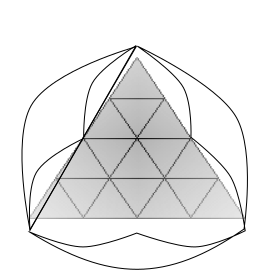
\includegraphics[width=0.2\linewidth]{triangleGraph.pdf} \qquad
\includegraphics[width=0.2\linewidth]{triangleGraphT.pdf} \qquad
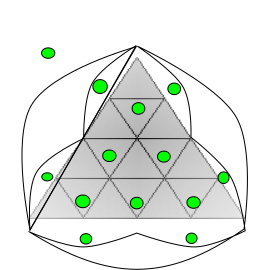
\includegraphics[width=0.2\linewidth]{triangleGraphF.pdf}

Note that the green circle not contained in any triangle signifies that the outer edges form a triangle. 

Note that we can increase this by doubling the side lengths, which will mean that the exposed sides will have additional edges connecting the three new ends. 

In general, $H_{n,p}$ does something similar, but with higher value cliques. The $p$ represents how tall the triangle is. 

Now that we have this, we can make an easy reduction from $1$-in-3 SAT. What we will do, is we will have copies of the above triangle graph that are large enough to contain many patches. By a patch, we mean the packing of the four triangles. 

We will call the graph $T$-partitioned if the partition looks like the middle one above in the topmost triangle, and $F$-partitioned if the partition looks like the far right one above in the topmost triangle. Note that we can divide $H_{3,p}$ into many patches, where each patch is an equilateral triangle of side length $2$. A $T$-patch is one with triangle pointing up and an $F$-patch is one with triangle pointing down. 

We will want to pick $p$ large enough so that there are many patches that are far away from each other. In particular, we want to have at least $3c$ patches a distance some constant, lets say 10. 

So now what we will have one $H_{n,p}$ for each variable, and three for each clause. Imagine stacking these on top of each other, and we will associate certain edges together with others in order to connect the graphs. We will ensure that the clauses have exactly one of the $H_{n,p}$ to be $F$-Partition, and by connecting them, we will make that corresponding variable $T$-partitioned if the variable appears in the clause, and $F$-partition if its negation appears in the clause. 

We will connect them by associating edges of patches. For example, for clauses, we will associate one $T$-patch in all of them, and remove the inner $T$-patch. This means that exactly one of the clauses must be partitioned into an $F$-partition. The other two $H_{n,p}$ which belong to the clause will have to be partitioned into a $T$-partition since we can think of the $T$-patch being filled since it ``belongs" to another part of the clause. 

Now if a variable appears in a clause, then connect one of clauses with the variable. We will connect by associating one $T$-patch of the clause with an $F$-patch of the variable. In some sense, this means flipping one of the graphs and making the path the same. If the clause is partitioned into an $F$-partition, this means that the $T$-patch has outer edges not filled by the clause, which means that the variable must fill them. Since it is connected to an $F$-partition, the variable must be $T$-partitioned. 

Likewise, if the negation of a variable appears, then we associate a $T$-patch of the clause to a $T$-patch of the variable. 

Therefore, if the 3SAT formula has a satisfying assignment where exactly one of the values per clause is true, then this graph has an edge partition into triangles. If it does not have a satsfying assignment, then we know that an Edge partition in on of the $H_{n,p}$ must be both $T$-partitioned, and $F$-partitioned, which is a contradiction.

\bibliographystyle{plain}
\bibliography{references}

\end{document}  
